\documentclass[]{article}
\usepackage[a4paper,includeheadfoot,margin=2.54cm]{geometry}

\usepackage{graphicx}
\usepackage{amsmath}
\usepackage{float}
%opening
\title{Pre-Covid (2019) Sofia Real Estate \\ 
	Econometric Analysis \\
	 of Market Conditions \\
	  R402 - Applied Econometrics I \\ AEEM cohort 2025/26 \\ Course Project}
\author{Riste Petrov}

\begin{document}

\maketitle

\begin{abstract}
	This econometric analysis examines the pre-COVID Sofia real estate market in 2019, utilizing a comprehensive dataset of 64,448 observations. The study aims to identify key determinants of property prices and develop predictive models for market conditions. Data manipulation involved refining variables such as property size, neighborhood location, and amenities, emphasizing geospatial accuracy through coordinate plotting and neighborhood management. The analysis incorporates a hedonic pricing framework, considering factors like proximity to metro stations, parks, shopping malls, and essential services, alongside property attributes such as construction type, age, and heating facilities. Price transformations, including logarithmic adjustments, were applied to improve model fit. Regression models—both structural and non-structural—were estimated to assess property valuation and the likelihood of properties being over- or underpriced, with logistic models achieving an accuracy of approximately 88\%. Limitations include multicollinearity and model misspecifications, acknowledged through variance inflation factors and heteroscedasticity tests. Despite these issues, the models demonstrate significant predictive power, offering valuable insights into Sofia’s market dynamics. This research underscores the importance of precise geospatial data and comprehensive variable selection in real estate econometrics, providing a robust tool for market analysis and valuation prior to the disruptions caused by the COVID-19 pandemic.
\end{abstract}
\vspace{2em}
\tableofcontents
\newpage
\section{Introduction}

During the classes of Applied Econometrics I, several tasks were aimed to identify and address econometric problems inherent in various datasets. One of these datasets was utilized in this research paper (explained in detail in the introduction). Previously, we had an older dataset that employed a different methodology; during its exploration, we discovered that the location parameter was not properly surveyed and reported.\\

The issue stemmed from treating location as a logical categorization instead of a continuous variable. This approach deviated from the common practice of using vectors to represent each directional attribute, which led to outcomes that differed from those intuitively expected. In the new dataset, these issues were resolved through plotting and calculating each neighborhood's coordinates.\\


Furthermore, challenges related to the categorization of locations within neighborhoods are well-documented in the literature. Research argues that accurately surveying location as a continuous variable with vector representations is far superior to simplistic categorizations in hedonic pricing models (\cite{malpezzi2003}). Additional studies highlight that the location of a property influences not only its price but also the demographic and social dynamics of the surrounding neighborhood (\cite{bayer2004}).\\


Numerous studies have identified various factors that significantly influence property prices, aligning with the principles of hedonic pricing. For instance, central heating is a desirable feature that enhances comfort and energy efficiency, often leading to higher property valuations (\cite{freeman1974}). Proximity to metro stations provides residents with convenient transportation options, making it a key determinant of location desirability (\cite{malpezzi2003}). The age and construction type of a property also affect its market value; newer constructions typically incorporate modern amenities and technologies that command premium prices.\\


Moreover, properties located closer to the city center are often in higher demand due to their accessibility to employment opportunities, entertainment, and cultural amenities (\cite{case1989}). The proximity of essential services, such as kindergartens, further enhances the appeal for families, making such properties especially sought after (\cite{bayer2004}). Additionally, closeness to shopping malls not only adds convenience but also contributes to a neighborhood's overall attractiveness, positively impacting property values. These multifaceted influences underscore the importance of comprehensive data analysis in accurately assessing market dynamics and property valuations.\\


\newpage

\section{Base Dataset \& Data Manipulation}
The base dataset was full of \textbf{64,448} observations. The time-frame of capturing of the sample is between January 2019 \& December 2019 interpreted as an cross-sectional database with \textbf{14} baseline variables each presented followed with a short description below:
 

\begin{itemize}
	\item  type - referring to the size type of the property
	\item regiid - regional location of property in Bulgaria (useless - all observations are in Sofia)
	\item townid - the town where the property is located in(useless - all observations are in Sofia)              
	\item quartid - the neighborhood in which the property is located in
	\item price (Euro) - listed price
	\item area - area in square meter for the property
    \item euro/sq.m. - self-explanatory
    \item constr. - construction type (3 main types)
    \item year - construction year of the property
	\item floor - the floor at which the property is
	\item TEC - available central heating in the property
	\item published or renewed - date at which was listed. 
	\item valid\_date - date at which was delisted. 
	\item seller - type of the seller              
\end{itemize}

\subsection{Size Type}
\subsubsection{Base size type}
Size type was defined into 7 types. Two \& Three room apartments have a frequency of \textbf{$\approx$ 82\%} because of that they were assigned to be the baseline for the dummy selection, further more explained in section 3. Below is presented the histogram \& the distribution of Size Types could be viewed from the dataset:   \\
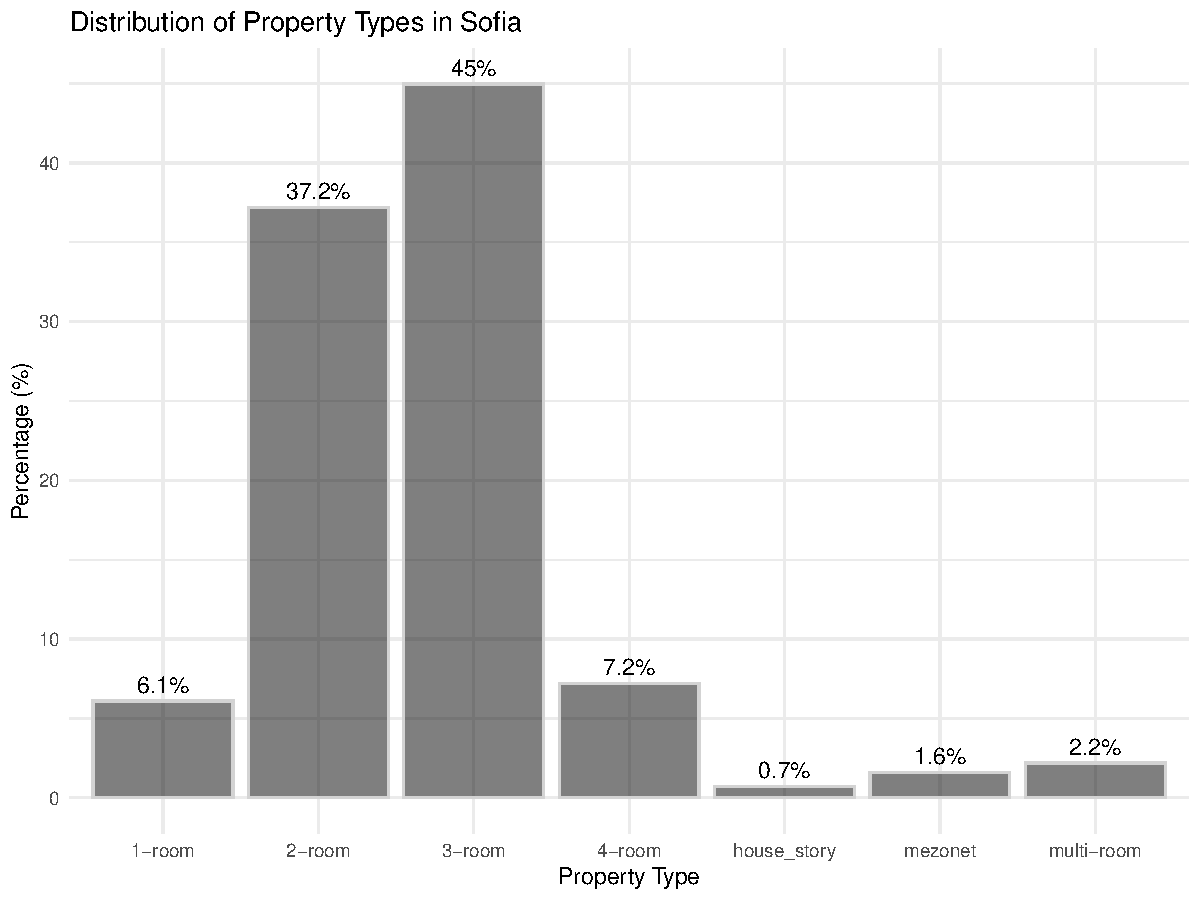
\includegraphics[width=\textwidth]{property_type_histogram.pdf}

\subsubsection{Modifications to Size Type}
In terms of data management, from the original dataset two new dummies were made:\\

Studio - which includes only the properties which are One roomed ones.

Story of a house - which includes only the properites which are story of a house.

Big property - which includes the size types - Four room \& Multi room apartments.


\subsection{Neighborhood}
\subsubsection{Quartid- base dataset}
Quartid  variable had unique 134 classifications and some variable without the classifier for neighborhood. 31 of these were excluded on the basis of various reasons as low frequency of observations bellow 0.01\% of total observations \& based on distance larger than the plotted map. (explained below)


\subsubsection{Neighborhood - management}
Because of the theory (mentioned in the Introduction) suggesting that categorical classification of neighborhood is inefficient, a custom approach was taken from the dataset, the similar approach was developed for each Neighborhood related engineered variable.\\
Ideally each observation should have address which could be pinpointed to a coordinate in the NS and WE axis, this could increase the accuracy of each other dummy variables.
\begin{center}
	\scriptsize
	Note: This approach of data gathering is expensive to maintain and difficult to control for inaccuracies of reported properties
\end{center} 

\subsubsection{Neighborhood Location \& Proximity to the Center}
As previously discussed, to achieve efficiency with the given dataset, a prop neighborhood map was made consisting of 500 by 500 meter squares in which the city of Sofia was plotted. Some of the neighborhoods (about 200 observations) which were too far away from the map or had tiny frequency in the sample were omitted from the map and the variables mentioned. The plotting was done using Google Maps \& Earth (the bounds of the individual Neighborhoods) in Libre Calc (Microsoft Excel), so the accuracy and objectivity is not up to standard but for this illustrative purpose was evaluated to be suitable. We can get into discussion that the neighborhood location is subjective, as neighborhoods tend to be merged, split and constructed over time.\\

Despite these limitations, it provided better results than the standalone categorical classification and offered some interesting insights into each variable. Below, the generated map featuring the 103 neighborhoods used is presented.

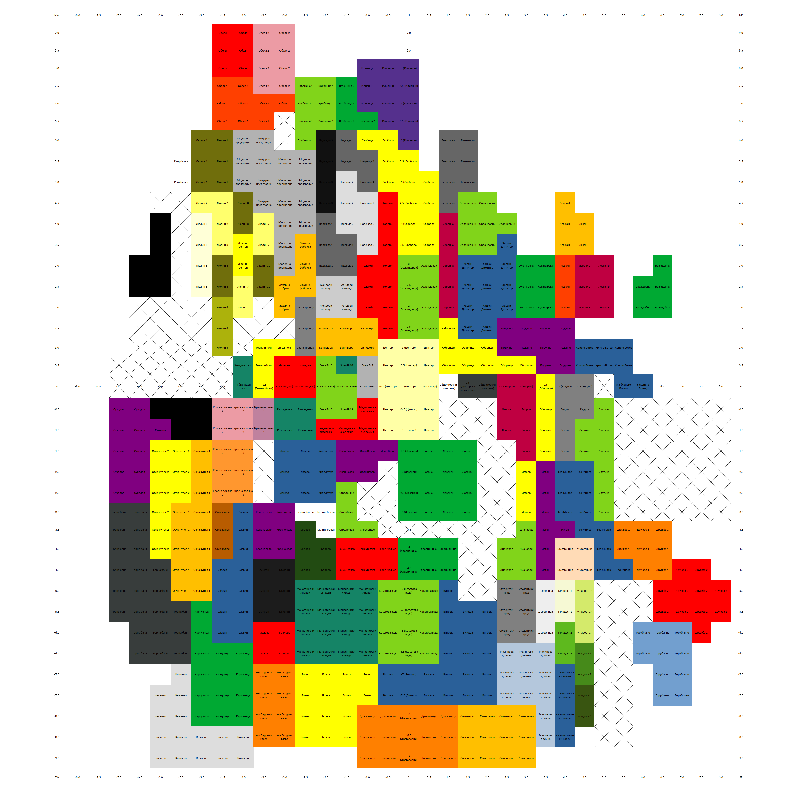
\includegraphics[width=\textwidth]{map.pdf}
\begin{center}
	\scriptsize
	Note: Color selection is random in order to differentiate neighboring neighborhoods.
\end{center}

To quantify the displayed map, a North-South (NS) and West-East (WE) coordinate system was established to determine a central point for neighborhood locations \& distance from center respectively.\\

This method assumes that property dispersion is evenly represented, allowing for effective analysis of property trends in each neighborhood, without exact coordinates for each observation (which  is not available).\\

The coordinates are distributed from -9 to 9 along both the NS and WE axes. The central point is defined as follows: \\

\begin{equation*}
	\text{NS} = \frac{-\text{NP}+\text{SP}}{2} - \text{CP}
\end{equation*}
\begin{itemize}
	\scriptsize
	\item[] NS - North - South central coordinate
	\item[] NP - most northern point in the neighborhood
	\item[] SP - most southern point in the neighborhood
	\item[] CP - central point of the city center along the NS axis
\end{itemize}

\begin{equation*}
	\text{WE} = \frac{\text{WP}+\text{EP}}{2} - \text{CP}
\end{equation*}
\begin{itemize}
	\scriptsize
	\item[] WE - West - East central coordinate
	\item[] WP - most western point in the neighborhood
	\item[] EP - most eastern point in the neighborhood
	\item[] CP - central point of the city center along the WE axis
\end{itemize}
\begin{center}
	\scriptsize
	Note: In real-life applications using global coordinates, the values for NP and WP would be affected by their position relative to the Greenwich Meridian and the Equator. If the neighborhood lies to the south of the Equator, NP may be negative, and if it lies to the west of the Greenwich Meridian, WP may also be negative.
\end{center}

The distance from the City Center from the central point is calculated as the diagonal line from the NS and WE coordinates, using the Pythagorean theorem for distance from the center: \\

\begin{equation*}
	\text{Distance from center} = \sqrt{\text{NS}^2+\text{WE}^2}
\end{equation*}

\subsubsection{Metro Availability}
This logical was determined for each tracked neighborhood, to determined if there was a metro station in the neighborhood which was within walkable distance (500 - 1000 meteres) of the center of the neighborhood. Approximately 2/3 of all neighborhoods had a positive value for metro access or $\approx$ 67\%. As of time of writing (2025), there is an ongoing expansion of the metro network which could negatively effect the effects of the metro variable, but that is a concern of future research.  


\subsubsection{Luxurious Locations}
Luxurious locations were set as a dummy variable based on a subjective or sentimental opinions with some basis from the average Euro per squared meter by neighborhood (defined in section 3.3 Price - management). Twenty neighborhoods were selected:

\begin{table}[H] % Allows placement here, at the top, bottom, or on a separate page
	\centering
	\caption{Luxurious Location Neighborhoods by Average Euros per Square Meter}
	\begin{tabular}{l r} % l aligns left, r aligns right
		\hline
		\textbf{Neighborhood}               & \textbf{Average Price (Euro/sqm)} \\ \hline
		Doktorski pametnik                   & 2,232.14                          \\ 
		Yavorov                             & 1,914.66                          \\ 
		Ivan Vazov                          & 1,838.22                          \\ 
		Izgrev                              & 1,600.00                          \\ 
		Iztok                               & 1,595.48                          \\ 
		Lozenec                             & 1,582.21                          \\ 
		Oborishte                           & 1,510.66                          \\ 
		Center                              & 1,470.00                          \\ \hline
		Boyana                              & 1,155.17                          \\ 
		Dragalevci                          & 1,105.68                          \\ 
		Manastirski livadi                  & 1,073.17                          \\ 
		Simeonovo                           & 1,000.00                          \\ 
	\end{tabular}
\end{table}
\begin{center}
	\scriptsize
	Note: As it could be noticed, Locations below Center in the table have lower Average Price but were included as they are in the south which is subjectively perceived to be more luxurious as it is more quiet, closer to mountain Vitosha \& the Buisness Center located in the south (which was underdeveloped before early 2010s) in a near proximity to Manastirski Livadi \& Mladost 4.
\end{center}


\subsubsection{Attractive Park Proximity}
Despite Sofia having several big Parks and many small Parks in almost all neighborhoods, the following three parks have been selected as "attractive" parks which are the most desired to visit during the weekends or are worth to visit them disregarding proximity as a factor. Below are presented the neighborhoods which are within walkable distance (500-1000 meters) from a park, in total 25 neighborhoods.

\begin{itemize}
	\item[] Boris Garden - Doktorski Pametnik, Yavorov, Lozenec, Center,
	Oborishte, Izgrev, Iztok
	\item [] South park - Lozenec, Ivan Vazov, Medical Academy,
	Strelbishte, Goce Delchev, Haldilnika, Vitosha
	\item [] Western Park - Gevegeliski, Zapaden park,
	Lylin 4/6/7/10, Zaharna Fabrika, Sveta Troica, Ilinden, Banishora
\end{itemize}

\begin{center}
	\scriptsize
	Note: Lozenec is on a walkable distance from two attractive parks, despite that the Park dummy doesn't give additional benefit of being to two parks instead of one.  
\end{center}

\subsubsection{Kindergarten Availability}
In regards of Kindergarten availability, was taken a dataset from the city of Sofia for 2019 - 2020 which listed all public Kindergartens which were in the neighborhood. There were about 190 kindergartens, some within the whole Sofia area which were not included, also an exclusion of private kindergartens was made as that data is not easily accessible in an aggregate format \& also because of the factor of the accessibility to them from economic standpoint doesn't make them a plus in considering buying a property.\\   

The Sofia city database of public kindergartens had many variables, specificlly 4 variables were selected to be a factor effecting property price.

\begin{itemize}
	\item[] Kids enrolled - number of kinds enrolled per neighborhood
	\item[] Number of kindergartens - in the neighborhood
	\item[] Density of kids per kindergarten - in the neighborhood
	\item[] Kindergarten (dummy) - if there is any kindergartens in the neighborhood
\end{itemize}

Approximately 70\% of the neighborhoods had a public kindergarten in the neighborhood.   

\subsubsection{Shopping Malls}
As theory hints (discussed in the Introduction) Shopping Malls have effect on significant effects on the hedonistic models of predicting the price of real estate. To justify it for our database, there are some minuscule negative externalities such as light, sound, air pollution \& traffic congestion but they have larger positive externalities such as proximity for middle class people to get employment in a near proximity to their homes. The following biggest and most visited shopping malls have been selected into the dummy variable, despite Sofia having smaller shopping malls in almost each neighborhood.\\


List of shopping malls selected \& neighborhoods in a walkable proximity (500-1000 meters) to them: 
\begin{itemize}
	\item[] Park Center - Lozenec, Ivan Vazov
	\item[] Bulgaria Mall - Manastirski Livadi, Borovo, Goce Delchev
	\item[] Western Mall - Lyulin 6/8/9, Gevgeliski, Zapaden Park, Sveta Troica
	\item[] Mall of Sofia - Zona B-5/18/19, Center, Banishora
	\item[] Serdika Mall - Reduta, Yavorov, Oborishte, Podulyane, Geo Milev
	\item[] The Mall - Mladost 1/1A, Druzhba 1, Drvenica
	\item[] Ring Mall - Mladost 3/4, Malinova Dolina, Amerikanski Koledzh
\end{itemize}

\subsubsection{Other possible variables}
In the process of conducting this research, several other location based factors were considered such as proximity to an industrial zone, airport, etc. Might have negative externalities, which could be subject for future research.\\

In the case of Sofia, proximity to the Airport is not applicable, because of the proximity of the Airport to the city Center, and most of the neighborhoods of the city  have negative externalities to some extent such as light and sound pollution from the Airport.\\

In my opinion the neighborhoods in close proximity to the airport are being developed as of time of writing (2025) despite of the stronger negative externalities because of \textbf{strong demand} for real estate, but a possible future correction of prices shouldn't be dismissed. 



\subsection{Price (in Euro)}
\subsubsection{Base dataset for the  Price variable}
Which is the main objective of the analysis \& regressions/models, to predict the price of an property.\\

Descriptive statistics:
\begin{itemize}
	\item[] Maximum value: 250,000
	\item[] Minimum Value: 11,753
	\item[] Mean value: 107,251.93
	\item[] Median (Absoloute Deviation): 43,893.85
	\item[] Standard Deviation: 47,670.17
	\item[] Skewness: 1.26
	\item[] Kurtosis: 3.25
\end{itemize}

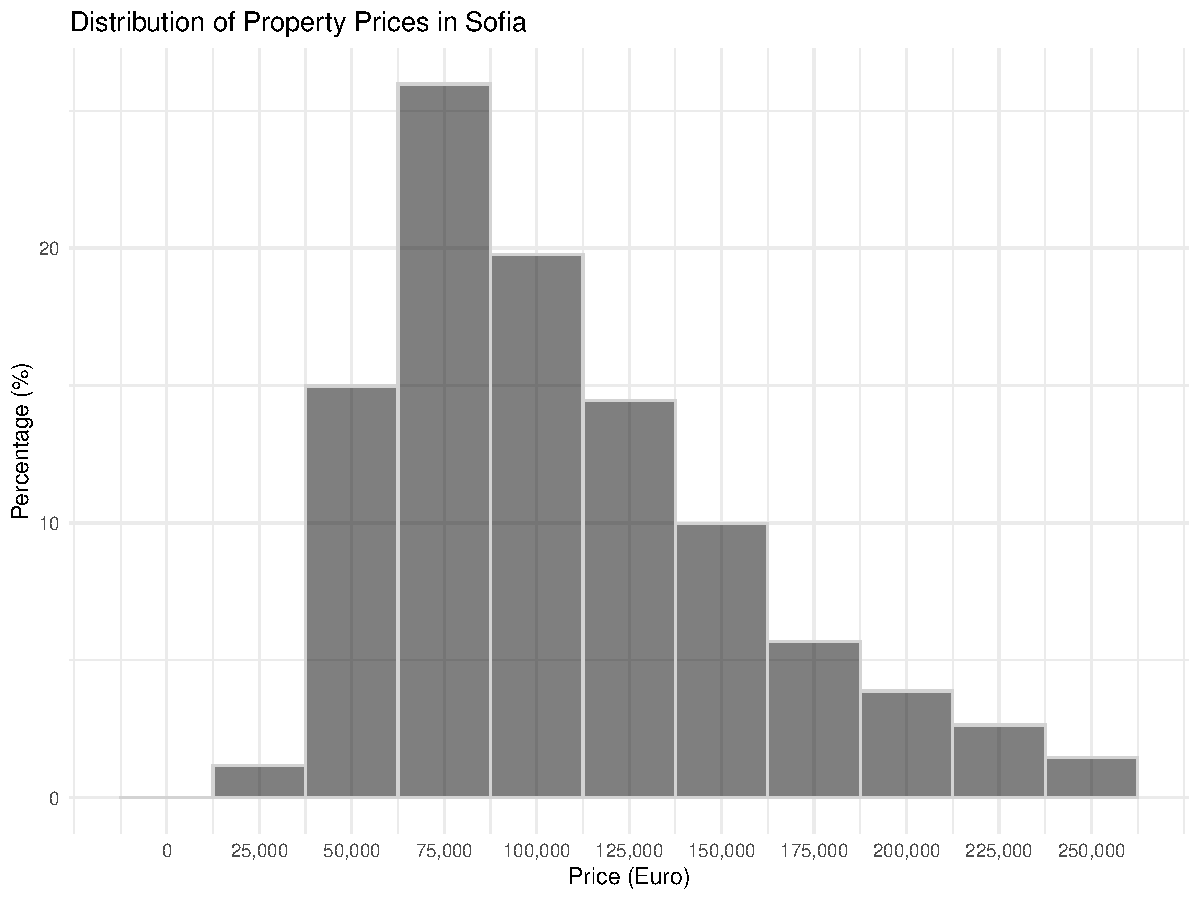
\includegraphics[width=\textwidth]{price_histogram.pdf}
\begin{center}
	\scriptsize
	Note: scale is adjusted for readability, doesn't represent the shape of the distribution as unadjusted histograms do. 
\end{center}
\subsubsection{Modifications on the Price variable}

In order to get more prices price predictability and practical significance transformations on price and price per square meter was transformed into a natural log.

\subsection{Area}
Descriptive statistics:
\begin{itemize}
	\item[] Maximum value: 300
	\item[] Minimum Value: 15
	\item[] Mean value: 94.61
	\item[] Median (Absoloute Deviation): 32.61
	\item[] Standard Deviation: 37
	\item[] Skewness: 1.26
	\item[] Kurtosis: 5.63
\end{itemize}

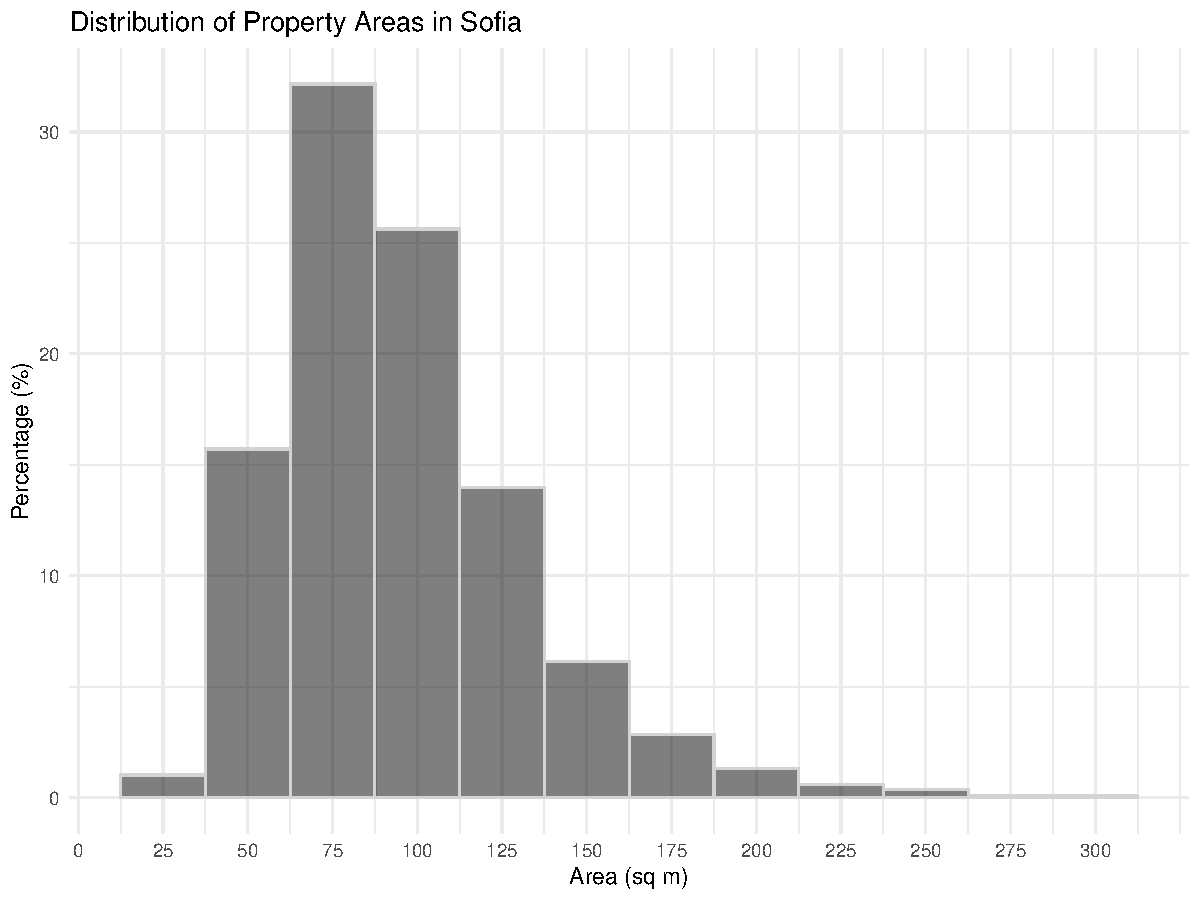
\includegraphics[width=\textwidth]{area_histogram.pdf}
\begin{center}
	\scriptsize
	Note: scale is adjusted for readability, doesn't represent the shape of the distribution as unadjusted histograms do. 
\end{center}

\subsubsection{Area - management}
natural logs of area variable weren't made because of the way of interpreting area as a factor on the price. People tend to think about area in terms of number of rooms or exact amounts instead of percentages. \\

The only two modifications were the creation of area$^2$, calculation of average area per neighborhood \& the difference between the observation area and area mean of the neighborhood. No premium dummies were made regarding it, despite it being used in the regressions instead of area or area$^2$.

\subsection{Euros per Square Meter}
\subsubsection{Euros per Square Meter - Base dataset}
Descriptive statistics:
\begin{itemize}
	\item[] Maximum value: 3,787.87
	\item[] Minimum Value: 156.83
	\item[] Mean value: 1,149.21
	\item[] Median (Absoloute Deviation): 252.47
	\item[] Standard Deviation: 346.15
	\item[] Skewness: 1.70
	\item[] Kurtosis: 4.58
\end{itemize}

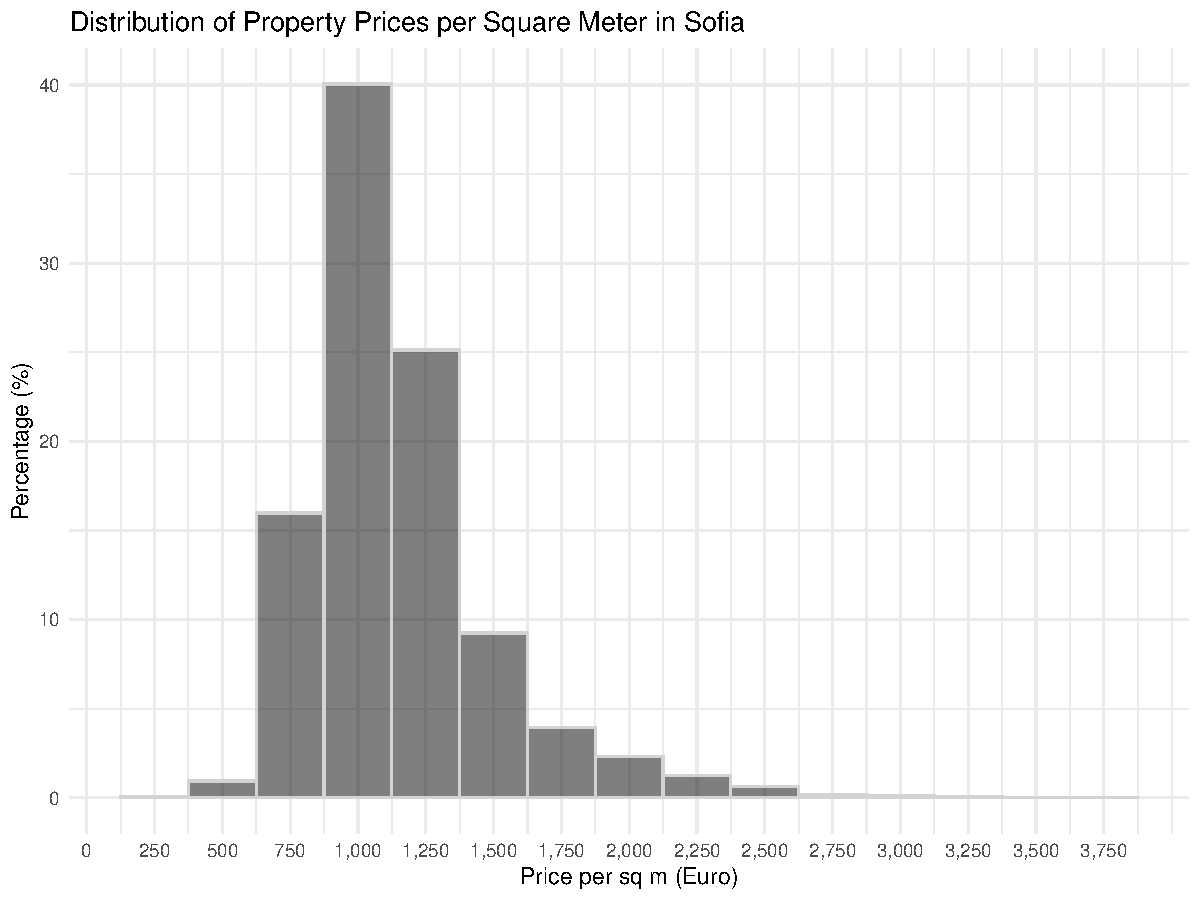
\includegraphics[width=\textwidth]{sq_m_histogram.pdf}
\begin{center}
	\scriptsize
	Note: scale is adjusted for readability, doesn't represent the shape of the distribution as unadjusted histograms do. 
\end{center}

\subsubsection{Euros per Square Meter - Management}

In order to get a better quantification and understanding for pricing in each neighborhood there were calculated averages \& medians for each neighborhood.\\

Regarding the distribution of the medians for each neighborhood the following Descriptive statistics were calculated:

\begin{itemize}
	\item[] Maximum value: 2,232.14 
	\item[] Minimum Value: 453.93
	\item[] Mean value: 1051.60
	\item[] Median (Absolute Deviation) : 187.77
	\item[] Standard Deviation: 453.93
	\item[] Skewness: 1.36
	\item[] Kurtosis: 6.60
\end{itemize}

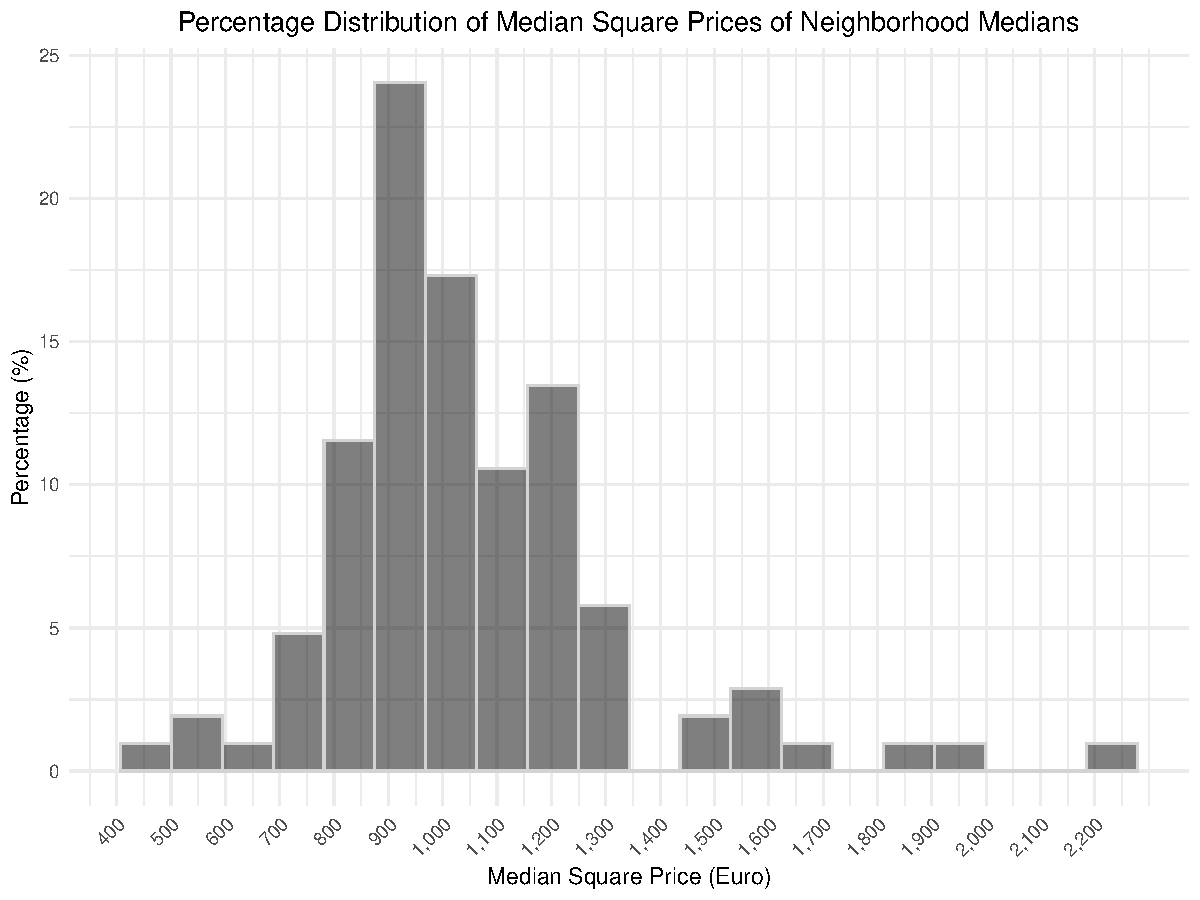
\includegraphics[width=\textwidth]{median_percentage_histogram.pdf}

 In order to use the distribution of the median price for each neighborhood a premium was calculated which is the difference between the observation price per square meter and the median of the respected neighborhood median price per square meter.\\
 
The descriptive statistics for the premium:
\begin{itemize}
	\item[] Maximum value: 2,199.22 
	\item[] Minimum Value: -1,202.38
	\item[] Mean value: -0.74
	\item[] Median (Absolute Deviation) : 180.63
	\item[] Standard Deviation: 254.20
	\item[] Skewness: 1.05
	\item[] Kurtosis: 7.76
\end{itemize}

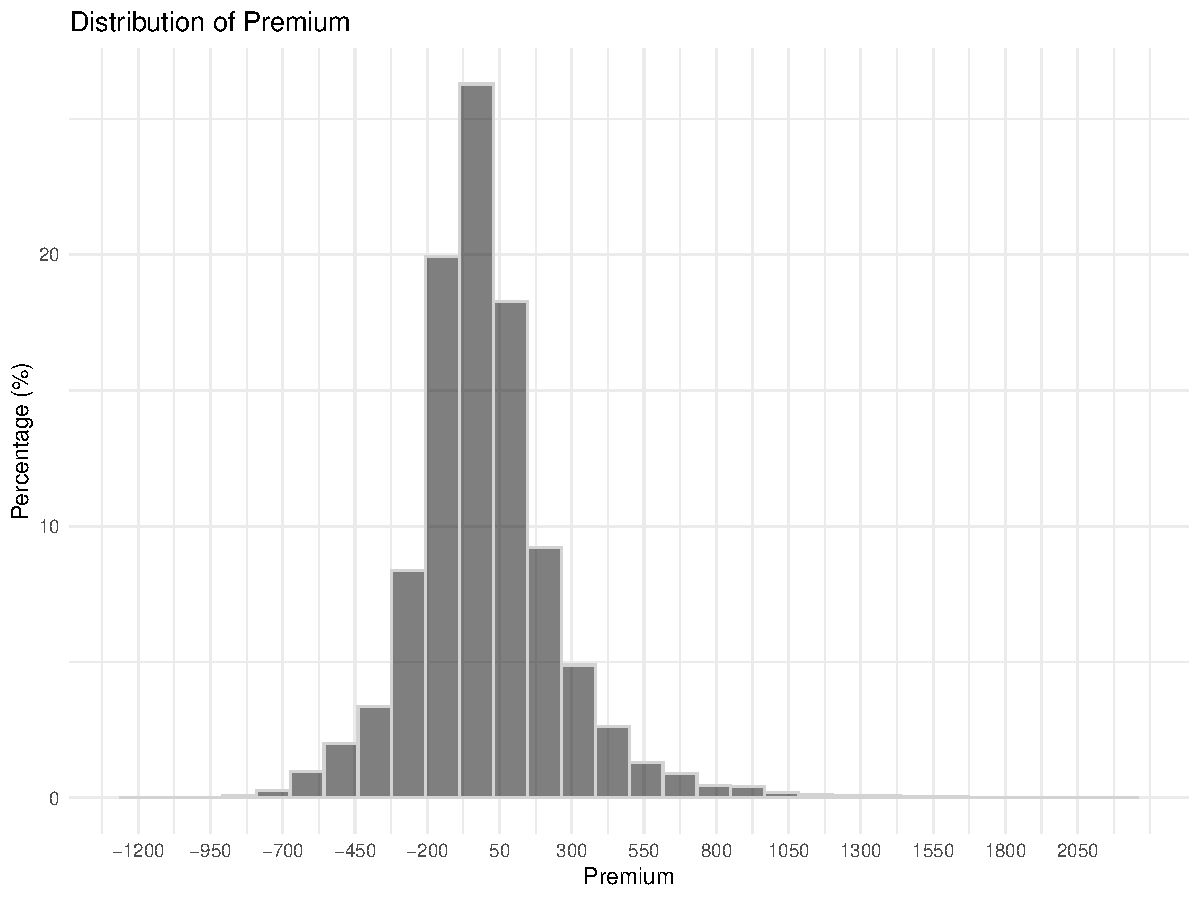
\includegraphics[width=\textwidth]{difference_from_median_histogram.pdf}

This premium variable and it's distribution was used to set dummy variables of Overpriced \& Underpriced. The dummies were assessed using a half standard deviation from the median away in both directions was representative for a possible inefficiently valued properties which resulted in:

\begin{itemize}
	\item [] $\approx$ 26\% were under-valued 
	\item [] $\approx$ 50\% were fairly-valued
	\item [] $\approx$ 22\% were over-valued
\end{itemize} 



\subsection{Construction type}
\subsubsection{Base dataset  - Construction type variable}

There were several miss-inputs into the raw database which were fixed, as it could be noticed most of the properties were constructed out of brick. (\textbf{$\approx$ 83\%}) Separate dummy was made for each construction type.  

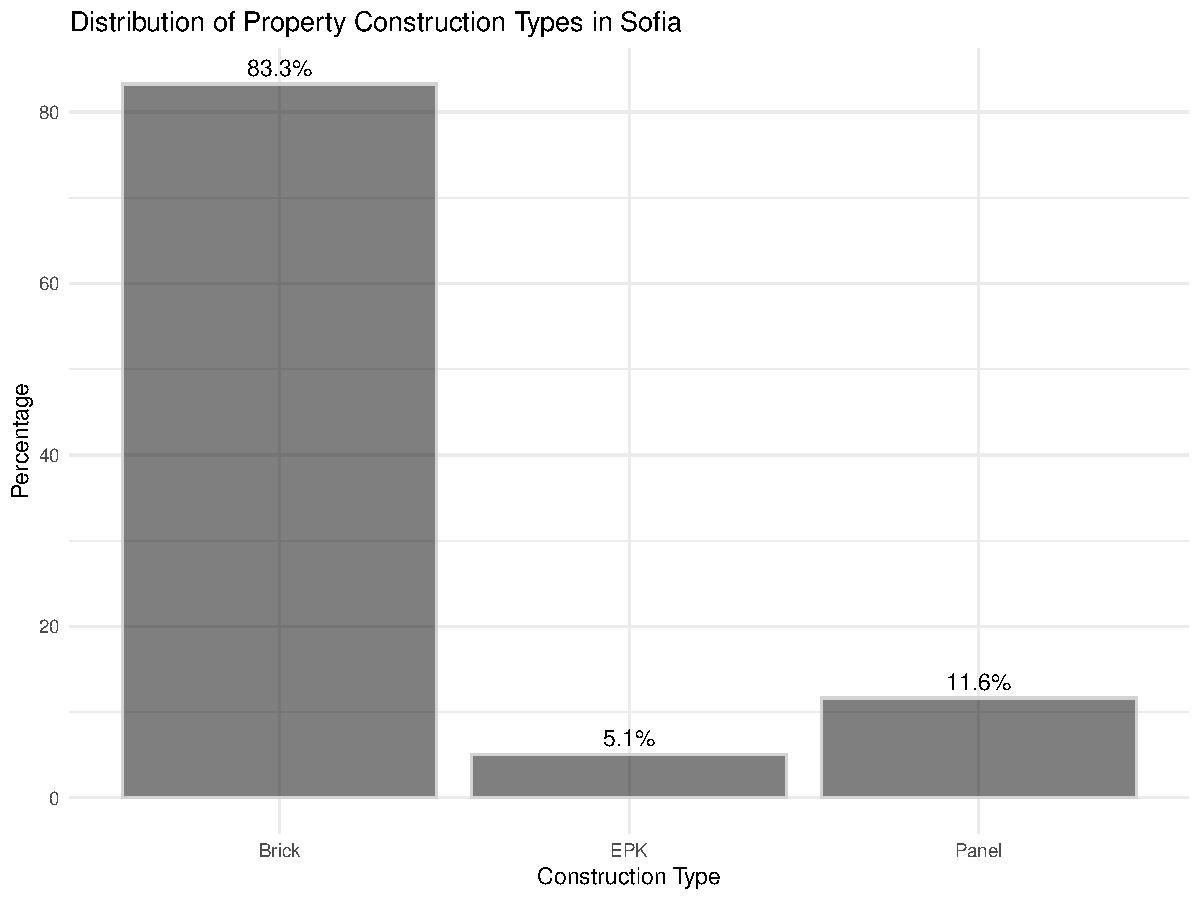
\includegraphics[width=\textwidth]{const_histogram.pdf}

In my opinion other crucial factors related for construction type, ideally should be focused towards gathering data of renovation if it was ever done, isolation (related to heating costs), recent upgrades to furniture (or it if it has at all furniture) \& similar long-term expenses related to construction and infrastructure.

\subsection{Year}
\subsubsection{Base dataset - Year}
The year variable was present in 42,424 observations or \textbf{$\approx$ 66\%} or 2/3 of  the observations had the year of the property reported. \\

Descriptive statistics excluding Not Available:
\begin{itemize}
	\item[] Maximum value: 2029 
	\item[] Minimum Value: 1862
	\item[] Mean value: 2003
	\item[] Median (Absoloute Deviation): 7.41 
	\item[] Standard Deviation: 22
	\item[] Skewness: -1.41
	\item[] Kurtosis: 4.58
\end{itemize}

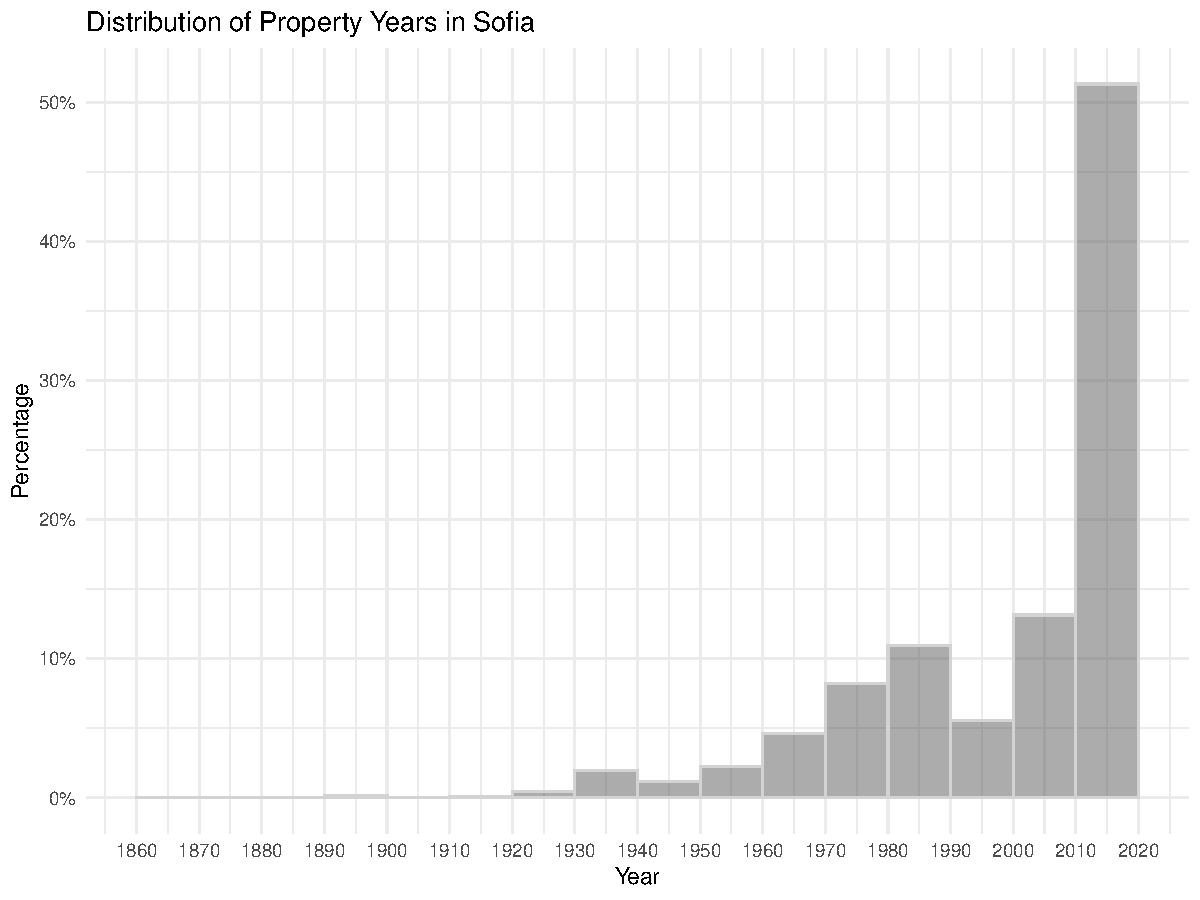
\includegraphics[width=\textwidth]{year_histogram.pdf}

\begin{center}
	\scriptsize
	Note: scale is adjusted for readability, doesn't represent the shape of the distribution as unadjusted histograms do. 
\end{center}

\subsubsection{Year - management}
The original year variable, was filtered for all missing observations. From that filtering calculation of neighborhood mean year was done from which it was calculated the difference from the observation and it's respective neighborhood. This was used in some of the diagnostic regressions, but didn't have any application in the presented regressions \\

Because of the distributions of the filtered year variable \& the difference, there was no need for a age-premium (despite it was created), but rather just an old variable was made. Which was based on the filtered year variable, by which each property older then 2004 was considered old. Which follows the economy of Bulgaria in terms of GDP and the effects from the crisis in the late 90s and the start of construction expansion since 2004.


\subsection{Floor}
The calculation of the descriptive values for it was based on a weighted basis of the counts of each floor, floor was notable not that significant factor. Maybe if there was a variable of an \textbf{elevator available} at the building would have been more explanatory.\\

Descriptive statistics:
\begin{itemize}
	\item[] Maximum value: -1 
	\item[] Minimum Value: 22
	\item[] Mean value: 3.91
	\item[] Median (Absoloute Deviation): 1.48
	\item[] Standard Deviation: 2.65
	\item[] Skewness: 1.37
	\item[] Kurtosis: 6.39
\end{itemize}

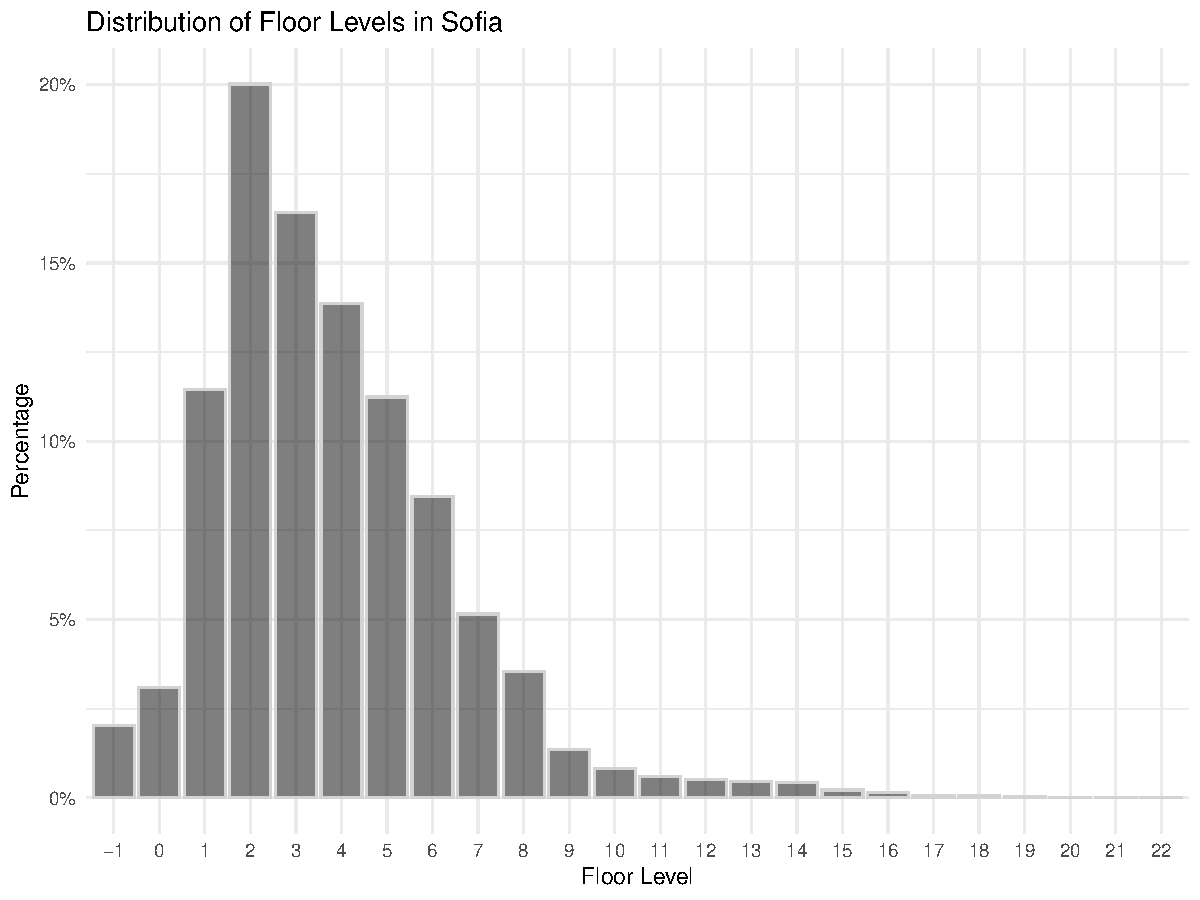
\includegraphics[width=\textwidth]{floor_histogram.pdf}

\subsection{Heating}
Heating was slightly modified in the functional form to accommodate the 0 \& 1 format. As described in section 4, it had some significance into the models used to predict the price of a property.
 
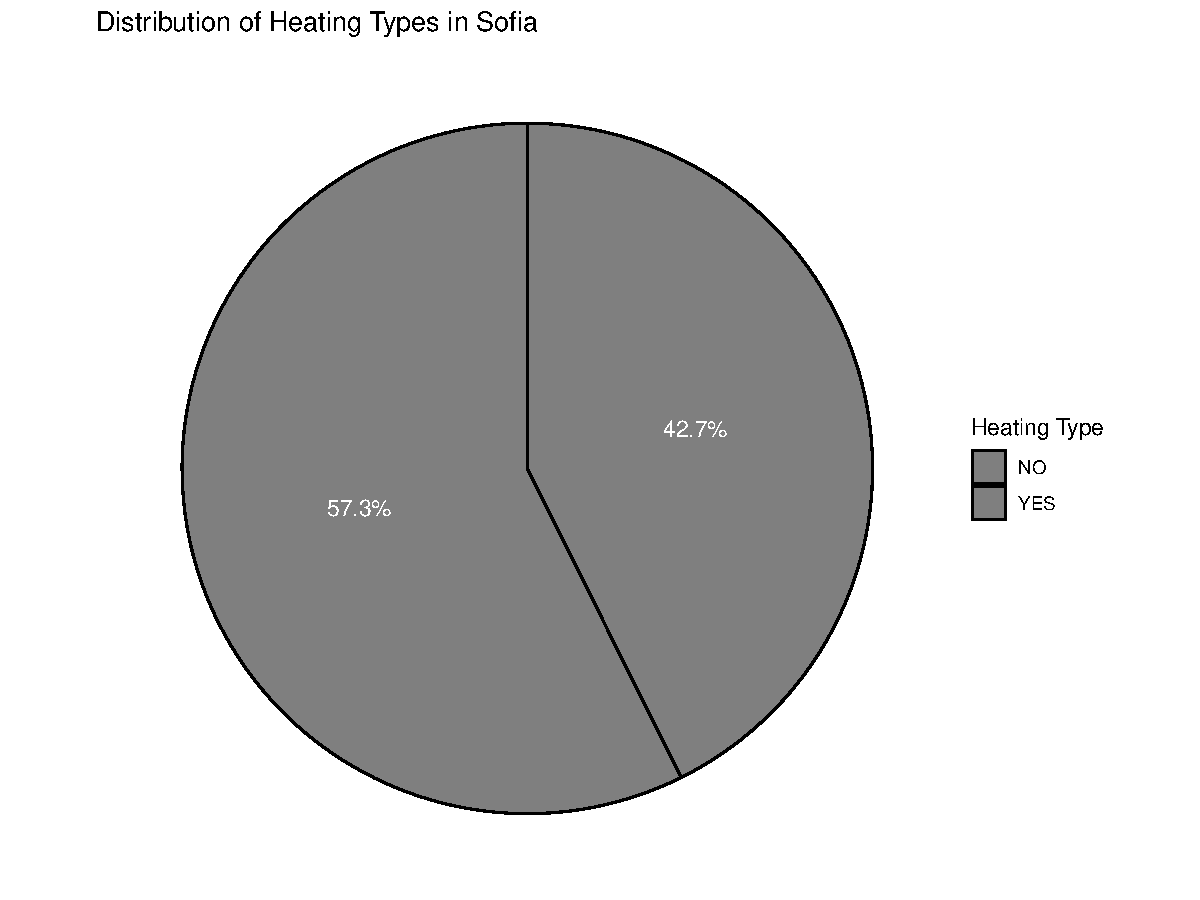
\includegraphics[width=\textwidth]{heating_pie_chart.pdf}

\subsection{Listing time}
Despite it had limited application in the presented regressions it was created based on the published date and valid date variables calculating their difference which should have had a potential desirability indicator. Indicating that more sought for properties would have shorter listing days and vice versa.\\

In my opinion this was not a good metric which the regressions proofed, because valid date wasn't defined as the date at which the property got sold but rather it was set by the seller, which could be abused to add artificial urgency to attract more potential buyers.

\newpage

\newpage
\section{Regressions \& Model}
As previously mentioned the analysis tried to describe the market conditions of the Sofia Real Estate market in 2019, but also had the main objective to build a model which will predict the  price of a property based on the provided dataset, with emphasis on location \& amenities near the location/neighborhood as major factors. 

\subsection{Structure of the Model}
Before the structural model approach was chosen, there were multiple regressions  developed with decent results of predicting the price without a need of any structure.\\

The structural approach was chosen with the main reason of utilizing a more real world application. This approach included endogen values for Over \& Underpriced variable using logit models for both variables.\\

 Which in practice would simulate an experienced \& knowledgeable  realtor, real estate agent or a valuator advising whetter a property is Overpriced or Underpriced in terms of the neighborhood location, far better than the average person and slightly better than the coin flip.\\
  Graphical representation of the model: \\


\begin{center}
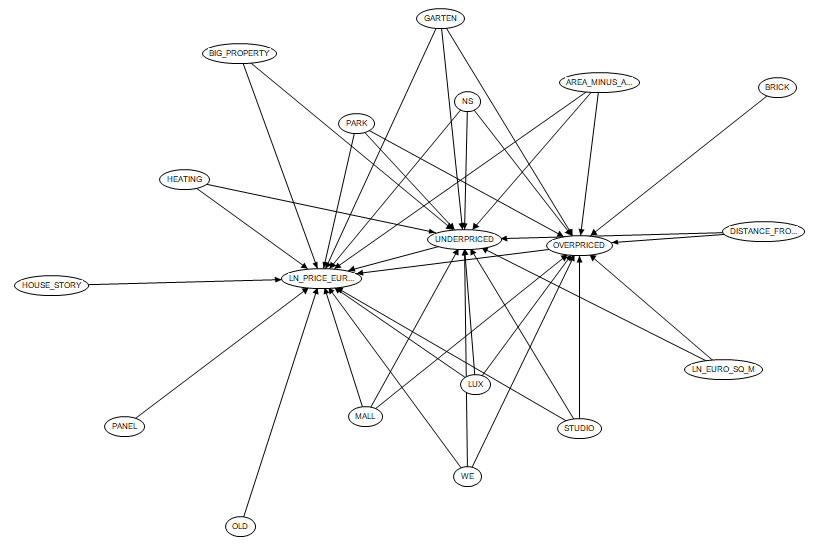
\includegraphics[width=\textwidth]{model-structure-2.png}

	\scriptsize
	Note: The experts mentioned usually don't have the best interest of the end client, as they have motivations stimulated by self interests such as sales/valuation commissions. Even licensed valuators in real world applications, in my humble experience have tinkered valuations in order to lower/raise tax and exposure.    
\end{center} 


\subsection{Logit Regressions for Overpriced \& Underpriced}
Before presenting the main structural model and the main regression using the Overpriced \& Underpriced as endogenous variables, follows explanation regrading them.\\

For the prediction regressions the cutoff point of probability was used at/near 1\% False Positive Rate or 99\% Specificity.\\

This was assigned at that level following the logic that the time cost of finding Overpriced or Underpriced properties is less important than the avoidance of making a wrong investment into a non Overpriced or Underpriced property.  


\subsubsection{Overpriced formula}
Prediction of Overpriced is determined by the following formula:

\begin{equation*}
	\text{Probability of Overpriced} = \frac{1}{1+e^{-(APREM+NS+WE+DFC+BRK+STUD+LUX+MLL+PRK+LNEUR)}}
\end{equation*} 

Abbreviation explanination of products of coefficients and the respective values:
\begin{itemize}
	\item[] APREM - Area Premium (Observation Area - Average Area in Neighborhood)
	\item[] NS - North-South coordinate for the neighborhood
	\item[] WE - West - East coordinate for the neighborhood
	\item[] DFC - Distance from Center
	\item[] BRK - Brick dummy
	\item[] STUD - Studio dummy
	\item[] LUX - Luxurious location dummy
	\item[] MLL - Shopping Mall dummy
	\item[] PRK - Park dummy
	\item[] GRT - Kindergarten number coeff
	\item[] LNEUR - Natural Log Euro
\end{itemize}

\subsubsection{Overpriced regression}
\begin{table}[h!]
	\centering
	\caption{Regression Results for Overpriced}
	\begin{tabular}{lrccr}
		\hline
		Variable & Coefficient & Std. Error & T-statistic & Probability \\
		\hline
		C                      & -146.4141 & 1.4149 & -103.4802 & 0         \\
		AREA\_MINUS\_AVG\_Q    & -0.0020   & 0.0006 & -3.3998   & 6.74E-04  \\
		NS                     & 0.3035    & 0.0059 & 51.1905   & 0         \\
		WE                     & -0.2713   & 0.0071 & -38.0121  & 0         \\
		DISTANCE\_FROM\_CENTER & 0.7895    & 0.0129 & 61.2907   & 0         \\
		BRICK                  & -0.3284   & 0.0448 & -7.3303   & 2.30E-13  \\
		STUDIO                 & 0.8015    & 0.0634 & 12.6387   & 1.29E-36  \\
		LUX                    & -2.0820   & 0.0507 & -41.0561  & 0         \\
		MALL                   & 0.4036    & 0.0405 & 9.9591    & 2.30E-23  \\
		PARK                   & -0.5656   & 0.0467 & -12.1223  & 8.04E-34  \\
		GARTEN                 & -0.3083   & 0.0113 & -27.3200  & 2.45E-164 \\
		LN\_EURO\_SQ\_M        & 20.1503   & 0.1953 & 103.1841  & 0         \\
		\hline
	\end{tabular}
\end{table}

\subsubsection{Underpriced formula}
Prediction of Underpriced is determined by the following formula:

\begin{equation*}
	\text{Probability of Underpriced} = \frac{1}{1+e^{-(APREM+NS+WE+DFC+STUD+LUX+MLL+PRK+HEAT+LNEUR)}}
\end{equation*} 

Abbreviation explanination of products of coefficients and the respective values:
\begin{itemize}
	\item[] APREM - Area Premium (Observation Area - Average Area in Neighborhood)
	\item[] NS - North-South coordinate for the neighborhood
	\item[] WE - West - East coordinate for the neighborhood
	\item[] DFC - Distance from Center
	\item[] STUD - Studio dummy
	\item[] LUX - Luxurious location dummy
	\item[] MLL - Shopping Mall dummy
	\item[] PRK - Park dummy
	\item[] GRT - Kindergarten number coeff
	\item[] HEAT - Central Heating dummy
	\item[] LNEUR - Natural Log Euro
\end{itemize}

\subsubsection{Underpriced regression}

\begin{table}[h!]
	\centering
	\caption{Regression Results for Underpriced}
	\begin{tabular}{lrccr}
		\hline
		Variable & Coefficient & Std. Error & T-statistic & Probability \\
		\hline
		C                      & 113.7220 & 1.0409 & 109.2509  & 0                    \\
		AREA\_MINUS\_AVG\_Q    & 0.0045   & 0.0005 & 8.8436    & 9.27E-19             \\
		NS                     & -0.4287  & 0.0069 & -62.0574  & 0                    \\
		WE                     & 0.3047   & 0.0060 & 50.5009   & 0                    \\
		DISTANCE\_FROM\_CENTER & -0.8541  & 0.0132 & -64.5582  & 0                    \\
		STUDIO                 & -0.2372  & 0.0659 & -3.5992   & 3.19E-04			  \\
		BIG\_PROPERTY          & 0.3170   & 0.0502 & 6.3137    & 2.72E-10             \\
		LUX                    & 2.7848   & 0.0443 & 62.8679   & 0                    \\
		MALL                   & -0.7417  & 0.0345 & -21.4875  & 2.04E-102            \\
		PARK                   & 0.7540   & 0.0373 & 20.2247   & 5.93E-91             \\
		GARTEN                 & 0.4103   & 0.0102 & 40.3932   & 0                    \\
		HEATING                & 0.1878   & 0.0322 & 5.8373    & 5.30E-09             \\
		LN\_EURO\_SQ\_M        & -16.3306 & 0.1486 & -109.9225 & 0                    \\
		\hline
	\end{tabular}
\end{table}



\subsubsection{Disclosure of limitations of the models}

Using price per square meter seems were intuitive to be considered as a predictor in rational thinking without considering any econometric application. Predicting if something is overvalued or undervalued without knowing it's sell price seems irrational especially for non-unique and relatively liquid items such as residential real estate where an appropriate alternative similar property is also listed.\\


But also the way overpriced and underpriced were defined gives us multicolinearity issues if OLS is used for predicting. The origin for the multicolinearity is inclusion of LN\_EURO\_SQ\_M, as it could be noticed by the Variance Inflation Factor tests done with the OLS versions of the same specification as the logit regressions.

\begin{table}[h!]
	\centering
	\caption{Overpriced OLS version: Coefficients and Variance Inflation Factors (VIF)}
	\begin{tabular}{lcrr}
		\hline
		Variable               & Coefficient Variance & Uncentered VIF & Centered VIF \\
		\hline
		C                      & 0.00                 & 1,197.75       & -            \\
		AREA\_MINUS\_AVG\_Q   & 1.46E-09             & 1.20           & 1.20         \\
		NS                     & 1.87E-07             & 2.70           & 1.96         \\
		WE                     & 2.56E-07             & 1.49           & 1.47         \\
		DISTANCE\_FROM\_CENTER & 7.70E-07             & 15.58          & 3.10         \\
		BRICK                  & 1.30E-05             & 7.27           & 1.22         \\
		STUDIO                 & 2.92E-05             & 1.20           & 1.12         \\
		LUX                    & 1.26E-05             & 2.42           & 1.73         \\
		MALL                   & 9.69E-06             & 2.63           & 1.57         \\
		PARK                   & 1.16E-05             & 2.59           & 1.73         \\
		GARTEN                 & 7.68E-07             & 3.47           & 1.65         \\
		LN\_EURO\_SQ\_M        & 3.43E-05             & 1,131.19       & 1.67         \\
		\hline
	\end{tabular}
\end{table}

\begin{table}[h!]
	\centering
	\caption{Underpriced OLS version: Coefficients and Variance Inflation Factors (VIF)}
	\begin{tabular}{lcrr}
		\hline
		Variable               & Coefficient Variance & Uncentered VIF & Centered VIF \\
		\hline
		C                      & 0.00                 & 1,200.79       & -            \\
		AREA\_MINUS\_AVG\_Q   & 1.83E-09             & 1.30           & 1.30         \\
		NS                     & 2.13E-07             & 2.64           & 1.93         \\
		WE                     & 2.97E-07             & 1.49           & 1.48         \\
		DISTANCE\_FROM\_CENTER & 8.78E-07             & 15.31          & 3.05         \\
		STUDIO                 & 3.39E-05             & 1.20           & 1.12         \\
		BIG\_PROPERTY          & 5.38E-05             & 1.15           & 1.11         \\
		LUX                    & 1.46E-05             & 2.42           & 1.72         \\
		MALL                   & 1.13E-05             & 2.63           & 1.57         \\
		PARK                   & 1.35E-05             & 2.59           & 1.73         \\
		GARTEN                 & 9.11E-07             & 3.55           & 1.69         \\
		HEATING                & 8.87E-06             & 2.20           & 1.25         \\
		LN\_EURO\_SQ\_M        & 4.07E-05             & 1,155.90       & 1.71         \\
		\hline
	\end{tabular}
\end{table}

Why these results don't give us notable issues and as it could be seen in the summary they give us edge in predicting better than random chance?\\

Because of having a partial correlation and also the difference of the distributions of the premium (on it's basis over and underpriced are defined) \& the natural log of property prices

\begin{figure}[h!]
	\centering
	\begin{minipage}{0.48\textwidth}
		\centering
		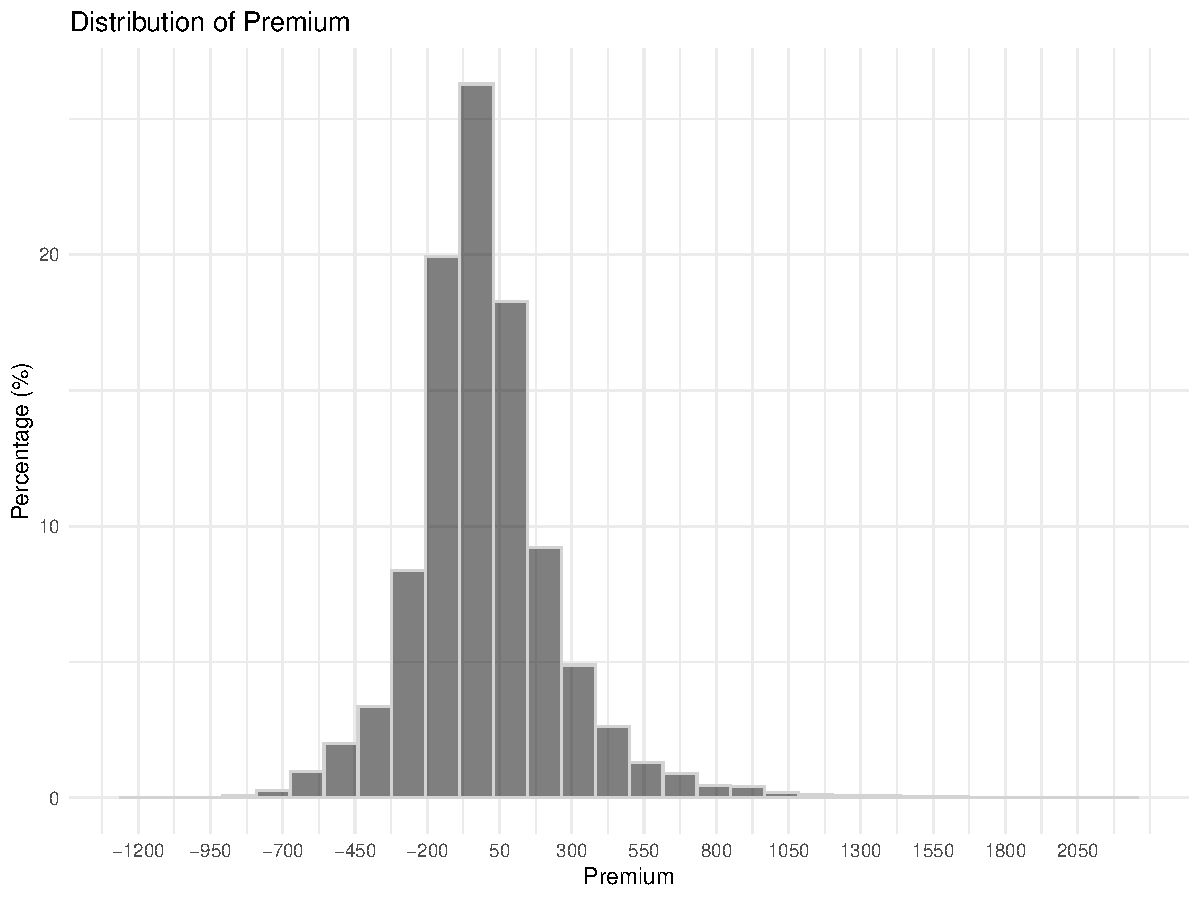
\includegraphics[width=\textwidth]{difference_from_median_histogram.pdf}
		\caption{Premium - Observation Price per Square Meter - Median for Neighborhood}
		\label{fig:diff_median}
	\end{minipage}\hfill
	\begin{minipage}{0.48\textwidth}
		\centering
		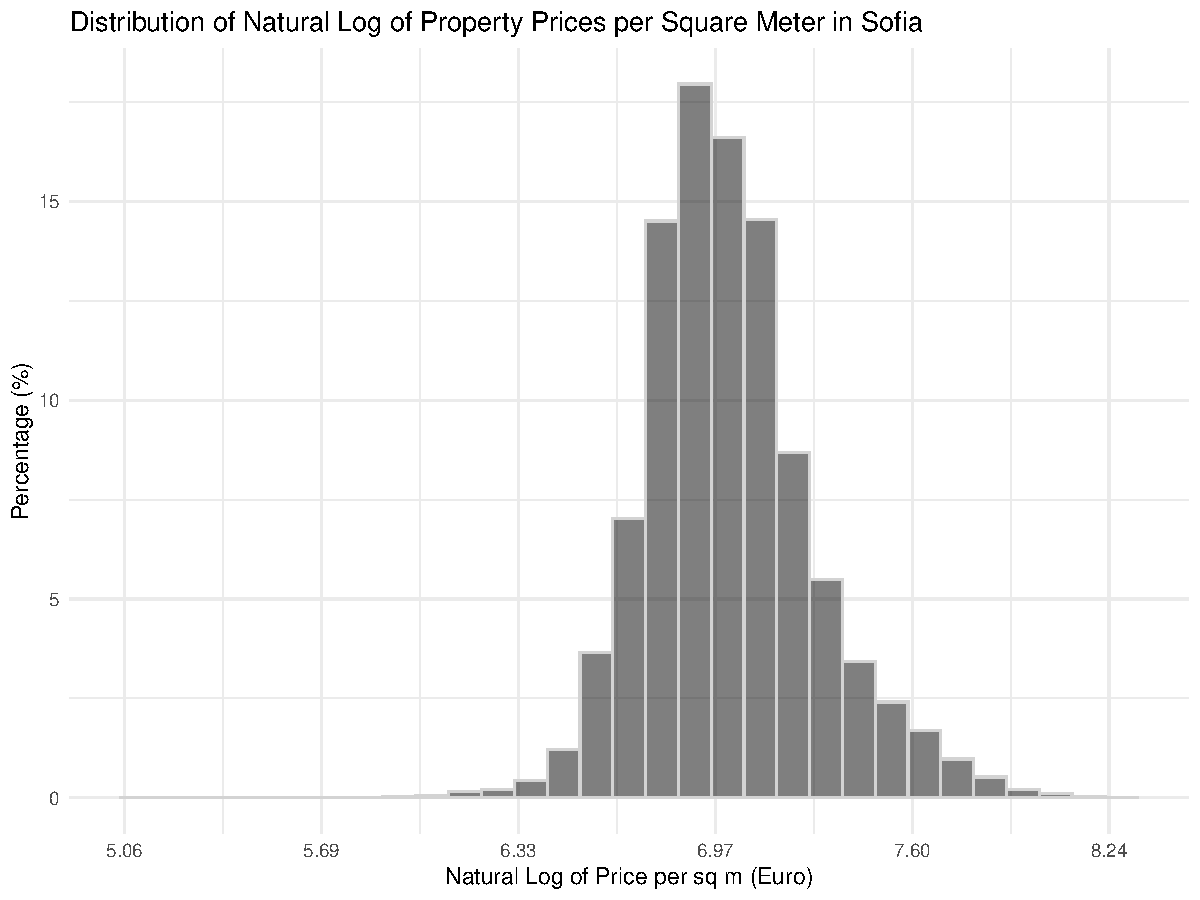
\includegraphics[width=\textwidth]{log_sq_m_histogram.pdf}
		\caption{Log of Square Meter Prices Histogram}
		\label{fig:log_sq_m}
	\end{minipage}
\end{figure}

\subsubsection{Summary for Logit regressions}
The Ramsis RESET Specificity test was conducted, concluding that the alternative hypothesis holds true, indicating that all available specifications resulted in the same misspecification outcome. Despite this, the following results were obtained based on the available dataset:

\begin{table}[ht!]
	\centering
	\caption{Performance Metrics for Overpriced and Underpriced Models}
	\resizebox{\textwidth}{!}{%
		\begin{tabular}{lrrrrrrr}
			\hline
			* FPR 1\%  & McFadden R² & AUC    & ABS Difference from 0.5 & Max Accuracy & Accuracy at *  & Diff from Max Acc * & Cut-off Probability for * \\
			\hline
			Overpriced  & 0.6142 & 0.4457 & 5.43\% & 91.15\% & 88.92\% & -2.24\% & 0.80 \\
			Underpriced & 0.5367 & 0.5747 & 7.47\% & 89.79\% & 88.43\% & -1.36\% & 0.71 \\
			\hline
	\end{tabular}}
\end{table}

In my opinion the models are suitable \& fulfill their real world role as an advisor with an edge of $\approx 5.5\%$ to $7.5\%$ (calculated in terms of Area Under the Curve metric) better property assessment than a coin flip or an cutoff adjusted accuracy of around 88\% of overall correct prediction. 


\subsection{Structural Model Regression versus Non-Structural Model Regression}

\subsubsection{Specification differences}
The main specification difference is usage of endogen values of overpriced and underpriced variables, also variables such as Big property dummy and Old were dropped because they became statistically insignificant \& if included would amplify the econometric (statistical) problems of the model.

\begin{table}[h!]
	\centering
	\caption{Model Coefficients and Statistics}
	\resizebox{\textwidth}{!}{
		\begin{tabular}{lcccccccc}
			\hline
			Variable & Coefficient & \underline{\textbf{Model Coeff}} & Std. Error & \underline{\textbf{Model STD}} & t-Statistic & \underline{\textbf{Model t-stat}} & Prob. & \underline{\textbf{Model Prob.}} \\
			\hline
			C & 11.2650 & \underline{\textbf{11.2757}} & 0.0018 & \underline{\textbf{0.0016}} & 6221.4476 & \underline{\textbf{7063.2024}} & 0 & \underline{\textbf{0}} \\
			AREA\_MINUS\_AVG\_Q & 0.0085 & \underline{\textbf{0.0087}} & 0.0000 & \underline{\textbf{0.0000}} & 237.7959 & \underline{\textbf{273.2812}} & 0 & \underline{\textbf{0}} \\
			NS & -0.0273 & \underline{\textbf{-0.0271}} & 0.0002 & \underline{\textbf{0.0002}} & -131.8707 & \underline{\textbf{-132.4238}} & 0 & \underline{\textbf{0}} \\
			WE & 0.0035 & \underline{\textbf{0.0033}} & 0.0003 & \underline{\textbf{0.0003}} & 10.5901 & \underline{\textbf{10.8713}} & 3.48E-26 & \underline{\textbf{1.67E-27}} \\
			GARTEN & 0.0282 & \underline{\textbf{0.0313}} & 0.0005 & \underline{\textbf{0.0005}} & 55.0116 & \underline{\textbf{68.1349}} & 0 & \underline{\textbf{0}} \\
			HEATING & 0.0392 & \underline{\textbf{0.0235}} & 0.0018 & \underline{\textbf{0.0017}} & 21.3752 & \underline{\textbf{14.0032}} & 5.15E-101 & \underline{\textbf{1.73E-44}} \\
			PANEL & -0.0369 & \underline{\textbf{-0.0274}} & 0.0039 & \underline{\textbf{0.0036}} & -9.4984 & \underline{\textbf{-7.6764}} & 2.20E-21 & \underline{\textbf{1.66E-14}} \\
			\textbf{BIG\_PROPERTY (EXCLUDED)} & \textbf{-0.0185} & \textbf{NA} & \textbf{0.0053} & \textbf{NA} & \textbf{-3.5108} & \textbf{NA} & \textbf{4.47E-04} & \textbf{NA} \\
			HOUSE\_STORY & -0.0664 & \underline{\textbf{-0.0627}} & 0.0123 & \underline{\textbf{0.0113}} & -5.3933 & \underline{\textbf{-5.5575}} & 6.94E-08 & \underline{\textbf{2.75E-08}} \\
			STUDIO & -0.3497 & \underline{\textbf{-0.3298}} & 0.0036 & \underline{\textbf{0.0035}} & -97.0671 & \underline{\textbf{-94.7580}} & 0 & \underline{\textbf{0}} \\
			LUX & 0.2694 & \underline{\textbf{0.2726}} & 0.0022 & \underline{\textbf{0.0019}} & 125.2937 & \underline{\textbf{144.7262}} & 0 & \underline{\textbf{0}} \\
			PARK & 0.1372 & \underline{\textbf{0.1396}} & 0.0018 & \underline{\textbf{0.0017}} & 76.0076 & \underline{\textbf{83.2489}} & 0 & \underline{\textbf{0}} \\
			MALL & -0.0358 & \underline{\textbf{-0.0370}} & 0.0020 & \underline{\textbf{0.0018}} & -17.7563 & \underline{\textbf{-20.2480}} & 2.28E-70 & \underline{\textbf{7.15E-91}} \\
			OVERPRICED (ENDOGEN) & 0.2538 & \underline{\textbf{0.3493}} & 0.0020 & \underline{\textbf{0.0021}} & 125.0280 & \underline{\textbf{166.9589}} & 0 & \underline{\textbf{0}} \\
			UNDERPRICED (ENDOGEN) & -0.2159 & \underline{\textbf{-0.3256}} & 0.0019 & \underline{\textbf{0.0020}} & -113.3328 & \underline{\textbf{-163.9697}} & 0 & \underline{\textbf{0}} \\
			\textbf{OLD (EXCLUDED)} & \textbf{0.0090} & \textbf{NA} & \textbf{0.0017} & \textbf{NA} & \textbf{5.4478} & \textbf{NA} & \textbf{5.12E-08} & \textbf{NA} \\
			\hline
		\end{tabular}
	}
\end{table}


The most distinct coefficient difference is the endogenvalues having of $\approx 50\%$ increase of coefficients (from 0.25 to 0.35 for overpriced). In regards to the intercept after the Log Log transformation it amounts to 78,884.14 EUR which realistically after adding neighborhood specific variables which are specific to the center. (PARK,MALL, LUX, GARTEN * 4) gives us a fairly priced flat in the city center which has an area of 93 meters squared priced at around  130,119,81 EUR. Which if compared by the median price of a 93,73 square meter flat (average area) it amounts (using median euro per square meter for the Center) to 137,783.10 EUR, which is only 5.5\% off the median price. 

\begin{table}[htbp]
	\centering
	\caption{Model Comparison Metrics}
	\begin{tabular}{lccc}
		\hline
		\textbf{Metric} & \textbf{Base} & \textbf{\underline{\textit{\textbf{Model}}}} & \textbf{Difference} \\
		\hline
		R-squared & 0.8016 & \underline{\textbf{0.8292}} & 0.0276 \\
		Adjusted R-squared & 0.8016 & \underline{\textbf{0.8292}} & 0.0276 \\
		S.E. of regression & 0.1956 & \underline{\textbf{0.1815}} & -0.0141 \\
		Sum squared resid & 2,441.6283 & \underline{\textbf{2,102.0733}} & -339.5551 \\
		Log likelihood & 13,579.9087 & \underline{\textbf{18,358.2952}} & 4,778.3865 \\
		F-statistic & 17,191.5111 & \underline{\textbf{23,834.1718}} & 6,642.6607 \\
		Prob(F-statistic) & 0.0000 & \underline{\textbf{0.0000}} & 0.0000 \\
		Prob(Wald F-statistic) & 0.0000 & \underline{\textbf{0.0000}} & 0.0000 \\
		Mean dependent var & 11.4878 & \underline{\textbf{11.4878}} & 0.0000 \\
		S.D. dependent var & 0.4392 & \underline{\textbf{0.4392}} & 0.0000 \\
		Akaike info criterion & -0.4251 & \underline{\textbf{-0.5749}} & -0.1498 \\
		Schwarz criterion & -0.4228 & \underline{\textbf{-0.5729}} & -0.1501 \\
		Hannan-Quinn criterion & -0.4244 & \underline{\textbf{-0.5742}} & -0.1499 \\
		Durbin-Watson stat & 1.6314 & \underline{\textbf{1.6243}} & -0.0070 \\
		Wald F-statistic & 15,293.1629 & \underline{\textbf{22,274.9111}} & 6,981.7481 \\
		\hline
	\end{tabular}
\end{table}

Inclusion of the endogeneity increases the ordinary \& adjusted R$^2$ by 2\%, increases the ordinary \& Wald F-statistics which shows a general better statistical significance of the model.

\subsubsection{Econometric problems}

As the dataset is cross-sectional type the problem of autocorrelation is disregarded as there is no time dimension analyzed.\\

\textbf{Multicolinearity}
As the diagnostic regressions were compiled, a corelation matrix was compiled which was made for cross checking if there are multicolinearity between variables of different groups of main variables.\\

Every iteration of the main model as it was evolving in the process of creation of modified variables, was tested using Variation Inflating Factor test. (VIF), to exclude any inter group variables which may be not critically correlated to the depended but on the VIF test would have shown drastically big results.

\begin{table}[H]
	\centering
	\caption{Coefficients Variance \& VIF for the Non Structural Regression}
	\label{tab:coef_vif}
	\begin{tabular}{@{}llll@{}}
		\hline
		\textbf{Variable}            & \textbf{Coefficient Variance} & \textbf{Uncentered VIF} & \textbf{Centered VIF} \\ \hline
		C                   & 3.28E-06    & 5.9928     &          \\
		AREA\_MINUS\_AVG\_Q & 1.28E-09    & 1.3038     & 1.2853   \\
		NS                  & 4.28E-08    & 1.9879     & 1.4871   \\
		WE                  & 1.07E-07    & 1.4282     & 1.3876   \\
		GARTEN              & 2.62E-07    & 3.4302     & 1.7793   \\
		HEATING             & 3.37E-06    & 2.4355     & 1.4097   \\
		PANEL               & 1.51E-05    & 1.1377     & 1.0894   \\
		BIG\_PROPERTY       & 2.78E-05    & 1.0836     & 1.0507   \\
		HOUSE\_STORY        & 1.51E-04    & 1.0219     & 1.0154   \\
		STUDIO              & 1.30E-05    & 1.2943     & 1.2243   \\
		LUX                 & 4.62E-06    & 3.1867     & 1.9616   \\
		PARK                & 3.26E-06    & 2.0615     & 1.3237   \\
		MALL                & 4.07E-06    & 3.2687     & 1.8091   \\
		OVERPRICED          & 4.12E-06    & 1.4700     & 1.1638   \\
		UNDERPRICED         & 3.63E-06    & 1.5627     & 1.1797   \\
		OLD                 & 2.72E-06    & 2.5712     & 1.1409   \\ \hline
	\end{tabular}
\end{table}
\begin{table}[H]
	\centering
	\caption{Coefficients Variance \& VIF for the Structural (Modeled) Regression}
	\label{tab:coef_vif_2}
	\begin{tabular}{@{}llll@{}}
		\hline
		\textbf{Variable}            & \textbf{Coefficient Variance} & \textbf{Uncentered VIF} & \textbf{Centered VIF} \\ \hline
		C                   & 2.55E-06    & 5.3497     &          \\
		AREA\_MINUS\_AVG\_Q & 1.02E-09    & 1.2199     & 1.2055   \\
		NS                  & 4.20E-08    & 2.0737     & 1.4287   \\
		WE                  & 8.95E-08    & 1.3289     & 1.3133   \\
		GARTEN              & 2.11E-07    & 3.2106     & 1.6435   \\
		HEATING             & 2.82E-06    & 2.4059     & 1.3646   \\
		PANEL               & 1.27E-05    & 1.1076     & 1.0621   \\
		HOUSE\_STORY        & 1.27E-04    & 1.0216     & 1.0152   \\
		STUDIO              & 1.21E-05    & 1.2500     & 1.1917   \\
		LUX                 & 3.55E-06    & 2.9175     & 1.7481   \\
		PARK                & 2.81E-06    & 2.1704     & 1.3314   \\
		MALL                & 3.34E-06    & 3.0286     & 1.6684   \\
		OVERPRICED\_CUTOFF  & 4.38E-06    & 1.3157     & 1.1185   \\
		UNDERPRICED\_CUTOFF & 3.94E-06    & 1.3571     & 1.1348   \\ \hline
	\end{tabular}
	
\end{table}


\textbf{Heteroscedacticity} 
In regards of heteroscedacticity it was concluded that heteroscedactitcity is present trough White's test \& Breusch-Pagan which were both conclusive about the heteroscedactity's presence in the regressions, because of that the White's robust standard errors where used as a remedy.


\subsubsection{Summary}
Despite the misspecification present of the structural model \& nonstructural regression confirmed  based on the especially the ones with using a cut-off fitted Ovepriced \& Underpriced values \& the dilema of the real estate professionals having different motivations than the buyers is a notable issue which could hinder efficiency in real life application of this model as an aid.\\

Professional and experience based judgment is \textbf{crucial}, but the model could be used with caution as a helpful tool for the professionals or ordinary property buyers as an second opinion checker when setting listing price or during sale negotiations.

\newpage
\section{Conclusion}

In conclusion, this study underscores the critical role of comprehensive data structure \& data management in advancing the accuracy of real estate valuation models. By capturing neighborhood location through continuous coordinates rather than simplistic categorical classifications, the research demonstrates that refined data collection significantly enhances model precision and reliability.\\


Furthermore, the analysis confirms that location-specific factors—such as proximity to the city center, parks, shopping malls, and kindergartens—alongside amenities like central heating and construction quality, are vital determinants of property prices. These findings highlight the importance of considering both geographic and infrastructural attributes when evaluating market values, as they substantially influence desirability and market dynamics.\\

The utilization of econometric modeling, particularly hedonic pricing approaches including logit regressions to predict over- and underpriced properties, illustrates the efficacy of these tools in market analysis. Achieving an accuracy of approximately 88\%, these models serve as valuable instruments for professionals and prospective buyers, offering data-driven insights that support more informed decision-making.\\


However, the research also recognizes inherent limitations and challenges, such as multicolinearity in the logit regressions, theoretical model misspecification, and data constraints—including subjective neighborhood classifications and potential biases in listing information. These issues suggest that while econometric models are beneficial, they require ongoing refinement and should be interpreted with caution.
\\

The implications for market practice are clear: models should complement, not replace, professional judgment. Incorporating additional variables—such as property renovation status, infrastructure projects, and real-time market shifts—could further enhance predictive capabilities in future research.\\


From a policy and investment perspective, data-driven models enable the identification of market inefficiencies, facilitating better investment decisions, urban planning, and policy formulation.\\


Finally, contextualized within Sofia’s 2019 market, the study illustrates how urban development, infrastructure expansion, and neighborhood attractiveness influence property prices. These insights provide a valuable snapshot of Sofia’s real estate landscape, with potential implications for its ongoing market evolution and strategic planning.\\



\end{document}


